\documentclass[conference]{IEEEtran}
\usepackage{amsmath,amssymb,booktabs,graphicx,microtype,cite,url,balance}
\usepackage[hidelinks]{hyperref}
\newcommand{\sisdr}{\mathrm{SI\text{-}SDR}}

\title{Causal Forecast-Conditioned BS-RoFormer\\for Ocean Sound Separation}
\author{\IEEEauthorblockN{Anonymous Authors}\IEEEauthorblockA{Anonymous Affiliation}}

\begin{document}
\maketitle

\begin{abstract}
We evaluate FC-BSR with one fixed main setting: a causal GRU, FiLM, a
BS-RoFormer separator, and 5-s windows.  Each supervised example is
$(H_t,N_t,s_t,x_t)$: twelve immediately preceding 5-s background features whose annotated whale-call intervals are
masked, an annotation-clean real 5-s ocean segment, a synthetic marine event,
and their exact mixture.  The available recordings provide 146.4 h of
call-free background, with 37.3 h eligible for training.  The 12-step GRU
reduces held-out forecast MAE from 2.111 to 1.926 dB (8.8\%) against
persistence.  On 4,096 held-out clean-background mixtures, FC-BSR is 0.134 dB
below the unconditioned separator (day-block 95\% CI $[-0.320,0.125]$), with no
detectable average improvement.  A separate 13-family study compares the other
conditioning modes as ablations.  On untouched real calls,
where no isolated stem exists, a frozen event classifier finds no clear
semantic advantage over the matched unconditioned separator.  We therefore
support fully supervised separation on annotated-clean backgrounds while
leaving the value of the forecast prior on unknown real events unresolved.
\end{abstract}

\begin{IEEEkeywords}
ocean acoustics, source separation, soundscape forecasting, BS-RoFormer,
weak-reference evaluation
\end{IEEEkeywords}

\section{Introduction}
Ocean backgrounds vary with shipping, weather, biology, and season
\cite{miksisolds2013indian}.  A mixture-only separator must infer both an
unexpected event and this changing background from the same observation.  We
instead ask whether the preceding soundscape can supply a causal prior.  Our
main data tuple is
\begin{equation}
\begin{aligned}
 &(H_t,N_t,s_t,x_t),\quad x_t=N_t+s_t,\\
 &H_t\xrightarrow{\mathrm{GRU}}\widehat S_t,\qquad
 x_t\xrightarrow[\widehat S_t]{\mathrm{FiLM+BSR}}(\hat s_t,\hat N_t),
\end{aligned}
\end{equation}
where $H_t$ excludes annotated call intervals and $N_t$ is a real current
no-call segment.  Training has exact stems, while the separator never receives
$N_t$ or $s_t$ as input.

Time-domain separators \cite{luo2019convtasnet,luo2020dprnn}, attention models
\cite{subakan2021sepformer,wang2023tfgridnet}, and band-split systems
\cite{luo2023bsrnn,lu2023bsroformer} provide strong mixture-only backbones.
Hybrid Transformers and MixIT broaden the architecture and supervision regimes
\cite{rouard2023htdemucs,wisdom2020mixit}, but do not test a forecast of the
upcoming background.  FiLM, cross-attention, and cross-modal separation
\cite{perez2018film,vaswani2017attention,zhao2018pixels} motivate three
interfaces.  Forecasting baselines range from recurrent to linear and
patch-based models \cite{salinas2020deepar,oreshkin2020nbeats,zeng2023dlinear,nie2023patchtst}.

Our contributions are: (1) FC-BSR,\footnote{Code and reproduction instructions:
\url{https://github.com/D-eval/ocean_noise_pred_splite}.} with a single
pre-registered main setting (GRU+FiLM+BS-RoFormer, 5 s); (2) a reproducible
annotation-aware construction of 146.4 h of current call-free ocean background
and event-masked 5-s histories; (3) a 13-family marine-aware event generator;
and (4) a frozen-classifier evaluation on untouched real calls.  TOL-domain,
conditioning-mode, time-scale, and unannotated-background strength studies are
reported as ablations rather than as the primary evidence.

\section{Method}
\subsection{Forecast and conditional separator}
The main history $H_t\in\mathbb R^{12\times30}$ contains 30-band log-power
features computed on twelve preceding 5-s windows; annotated calls and their
2-s guards are excluded.  Features are normalized using training data only.
A residual GRU predicts
\begin{equation}
 z_t=\operatorname{LN}(\operatorname{GRU}(H_t)),\quad
 \widehat S_t=S_{t-1}+g_\psi(z_t).
\end{equation}
Residual initialization represents persistence exactly; a learned predictor is
retained only if validation MAE improves upon persistence
\cite{gneiting2011pointForecast}.

The main FC-BSR maps the mixture STFT to band tokens $X_k$ and applies FiLM
before the axial Transformer:
\begin{align}
\widetilde X_k&=(1+\tanh\gamma_k)\odot X_k+\beta_k.\label{eq:inject}
\end{align}
The separator predicts an event stem; the ocean stem is the mixture residual.
Training combines waveform $L_1$ and multi-resolution complex-STFT losses.
Concatenation and cross-attention are alternative conditioning ablations, not
the deployed FC-BSR configuration.

\begin{figure*}[t]
\centering
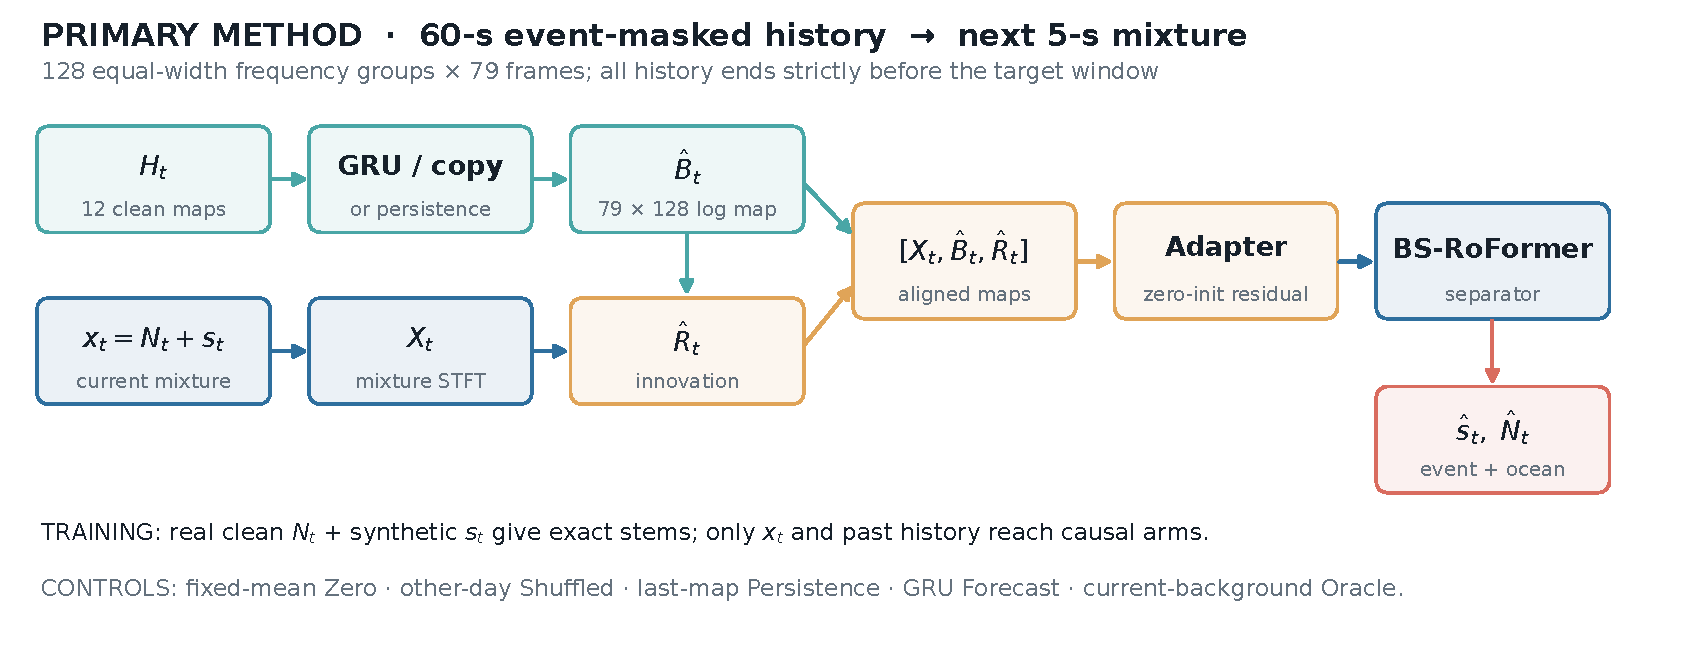
\includegraphics[width=.94\textwidth]{figures/architecture.pdf}
\caption{The fixed main setting and its supervised data tuple.  Event-masked
history drives the GRU forecast; real annotated-clean background and a
synthetic event form the current mixture.  FiLM conditions the BS-RoFormer and
the event estimate is supervised and the ocean estimate is its mixture-consistent residual.}
\label{fig:architecture}
\end{figure*}

\subsection{Marine-aware source distribution}
The generator contains 13 families: harmonic, linear chirp, inharmonic,
impulse train, frequency-modulated tone, band noise, whale upsweep, downsweep,
arch, S-curve, pulse packet, vessel tonal, and vessel cavitation.  Whale proxies
use one to three localized events with variable duration, curvature, partials,
taper, and flutter.  Vessel-tonal and narrow-band cavitation components draw a
5--20 Hz low-frequency-oscillator amplitude envelope with probability 0.8;
their broadband component is not modulated.  Training SNR is uniform on
$[-18,12]$ dB.  This distribution is intended to cover contour and modulation
patterns, not to claim species identity.

We quantify spectral displacement with directional $D_{\rm KL}(p\|q)$ and
finite symmetric Jensen--Shannon (JS) divergence \cite{lin1991divergence};
spectral entropy and source--ocean overlap are reported separately.  Larger
KL/JS expands coverage but is not treated as semantic diversity.

\subsection{Main data construction and secondary ablations}
The main dataset uses day-disjoint 2-kHz DCLDE 2013 recordings and whale-call
annotations \cite{gillespie2019dclde,shiu2020marine}.  Across 168 h of WAV,
excluding annotated calls and a 2-s guard on each side yields 146.4 h of
annotation-clean 5-s windows.  For each target, the 12 immediately preceding
5-s blocks from the same WAV form a 30-band history; a target is eligible only
when all history blocks are outside annotated calls and their 2-s guards.  This
avoids temporal averaging over an hour and forbids histories from crossing WAV
boundaries.  This leaves 94.5 h eligible overall, split into 37.3/9.7/47.6 h
for train/validation/test.
For each current clean $N_t$, a 13-family synthetic event $s_t$ is mixed to
form $x_t=N_t+s_t$.  The main split is by recording day, and the GRU receives
12 event-masked features from the immediately preceding 5-s windows.

Secondary ablations use NOAA--Navy SanctSound hourly TOL products
\cite{noaa2020sanctsound}.  MB03 deployments 01--02/03/04 are
train/validation/test.  Random-phase inversion creates controlled spectral
surrogates, not recovered audio.  Concatenation, cross-attention, KL/JS
coverage, and the one-hour history-resolution comparison are confined to this
domain.  The separate 42-h SanctSound WAV strength sweep also lacks event
annotations, so it is a useful controlled real-background ablation but is not
counted as clean-background primary evidence.

Complete-reference tiers report SI-SDR and SI-SDRi using scale-invariant
projection \cite{vincent2006sdr,leroux2019sdr}.  All uncertainty intervals are
seeded paired bootstraps, blocked by recording day for the main test.  The event classifier is frozen before any real-event
evaluation.  Current test features are used only as targets for the synthetic
full-reference task, never as GRU input; all histories end before $t$.

\section{Experiments and Results}
\subsection{Conditioning-mode ablation on spectral surrogates}
The primary architecture is fixed to FiLM.  Table~\ref{tab:ablation} compares
it with the alternative interfaces on controlled 5-s spectral-surrogate
examples; on 832 fixed-0-dB pairs (64 per family), FiLM improves 4.850 to
5.541 dB SI-SDRi.  Band-wise scale and bias directly modulate existing band
evidence.  Concatenation must compress doubled features, while cross-attention
must learn alignment from coarse predicted spectra under the same budget.

\begin{table}[t]
\caption{Conditioning-mode ablation on TOL-derived spectral surrogates (dB).}
\label{tab:ablation}\centering\footnotesize
\begin{tabular}{lrrr}
\toprule
Injection & Val. SI-SDRi & Test SI-SDRi & Paired $\Delta_0$\\
\midrule
None &4.864&4.059&0\\
Concatenation &5.343&4.432&+0.623\\
FiLM &\textbf{5.419}&\textbf{4.468}&\textbf{+0.692}\\
Cross-attention &5.128&4.261&+0.331\\
\bottomrule
\end{tabular}
\end{table}

FiLM gains 0.869, 0.835, 0.919, 0.906, and 0.806 dB on the five whale proxy
families.  Vessel tonal is the hardest family: the conditioned absolute
SI-SDRi is $-8.295$ dB, despite a 0.320-dB relative gain.  Overall gain has
weak correlation with JS ($r=-.057$) and entropy ($r=.122$), so increasing
divergence broadens support but does not predict usefulness.

\subsection{Primary fully supervised clean-background separation}
The main FC-BSR receives twelve event-masked preceding 5-s features and a current clean
5-s DCLDE segment; the 13-family event is added only after the clean background
is selected.  The model therefore sees $x_t$ and $H_t$, while the exact $N_t$
and $s_t$ are supervision.  The training split contains 37.3 h of
eligible clean current audio.  The 12-step GRU forecasts the next 5-s band
spectrum; validation MAE is 1.926 dB versus 2.111 dB for persistence (8.8\%
lower).
Table~\ref{tab:cleanmain} reports the held-out
full-reference comparison between the fixed main FC-BSR and its unconditioned
BS-RoFormer control.  The control shares data, initialization, optimizer,
training duration, and checkpoint selection.  Figure~\ref{fig:cleanstrength}
stratifies this paired test by injected SNR while retaining the fixed main
setting and held-out clean backgrounds.  Across 4,096 paired examples, FC-BSR
scores 9.497 dB SI-SDRi versus 9.631 dB for BS-RoFormer (paired difference
$-0.134$ dB, day-block 95\% CI $[-0.320,0.125]$); the average difference is
not distinguishable from zero.

\begin{table}[t]
\caption{Primary held-out clean-background + synthetic-event test.}
\label{tab:cleanmain}\centering\footnotesize
\resizebox{\columnwidth}{!}{%
\begin{tabular}{lrrr}
\toprule
Model & SI-SDRi (dB) & Target SI-SDR (dB) & Background SI-SDR (dB)\\
\midrule
BS-RoFormer & 9.631 & 6.479 & 10.061\\
FC-BSR (GRU+FiLM) & 9.497 & 6.345 & 10.155\\
\bottomrule
\end{tabular}
}%
\end{table}

\begin{figure}[t]
\centering
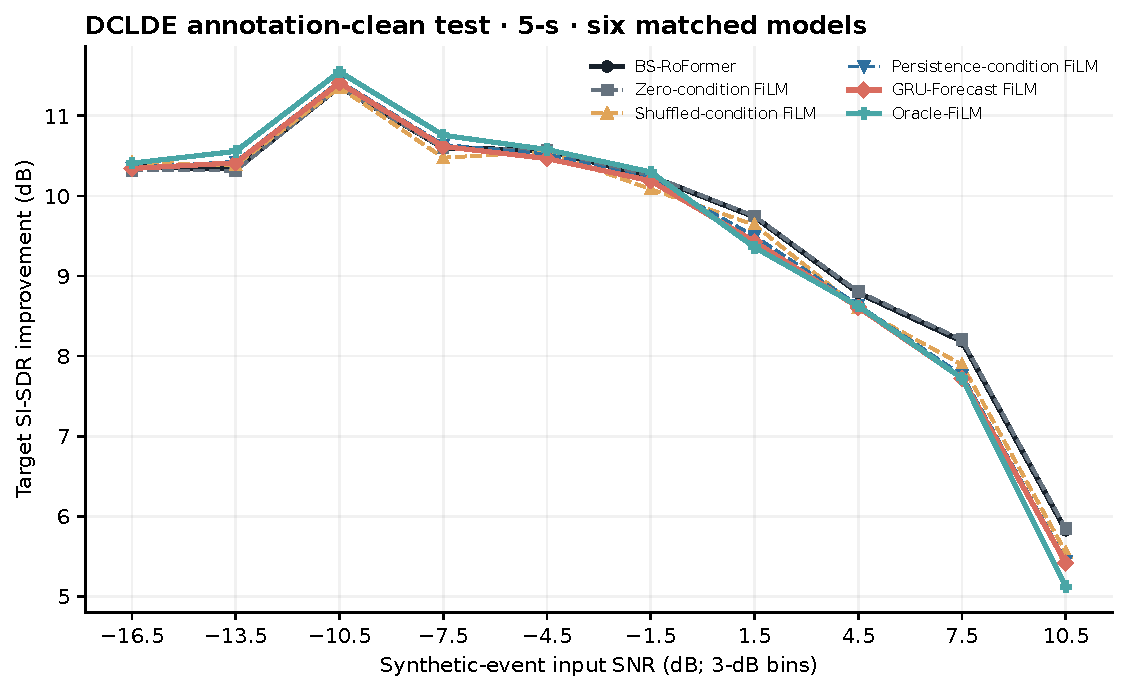
\includegraphics[width=\columnwidth]{figures/clean_background_strength.pdf}
\caption{Primary full-reference test on annotation-clean DCLDE backgrounds.
Target SI-SDRi is shown against injected event strength for matched BS-RoFormer
and FC-BSR; uncertainty is blocked by recording day.}
\label{fig:cleanstrength}
\end{figure}

\subsection{Secondary ablations: time scale and target strength}
The time-resolution diagnostic in Table~\ref{tab:windows} is an ablation on
continuous SanctSound audio, not the main annotation-clean data.  Only its
5-s predictor beats persistence on validation (MAE 1.366 versus 1.386 dB);
the other scales select persistence.  The separate 42-h strength curve also
uses unlabeled current background.  It shows that forecast conditioning is
strength-dependent in that domain and must not be read as a result on
annotation-clean current segments.

\begin{table}[t]
\caption{Ablation: predictor-resolution diagnostic on SanctSound background.}
\label{tab:windows}\centering\footnotesize
\begin{tabular}{lrrrr}
\toprule
Step & Predictor & Cond. & Base & Gain [95\% CI]\\
\midrule
5 s &GRU&29.753&28.527&1.226 [1.082,1.381]\\
30 s&Persist.&29.630&28.534&1.095 [0.935,1.265]\\
1 min&Persist.&29.661&28.533&1.128 [0.971,1.298]\\
10 min&Persist.&29.711&28.535&1.176 [1.036,1.326]\\
\bottomrule
\multicolumn{5}{l}{\scriptsize Cond./Base/Gain are target SI-SDRi in dB.}
\end{tabular}
\end{table}

The harder fixed-5-s experiment compares BS-RoFormer, current-spectrum oracle,
causal forecast, and time-shuffled condition on 1,152 paired test mixtures.
Averaged across training SNRs, the baseline scores 23.470 dB and Forecast-FC-BSR
22.871 dB ($\Delta=-0.599$, CI $[-0.851,-0.346]$); even the oracle is lower.
This exposes conditioning/capacity effects that the simpler diagnostic misses.
Figure~\ref{fig:strength} gives the more informative strength sweep.  Forecast
conditioning helps weak targets by 0.728, 0.643, 0.525, 0.366, and 0.157 dB at
$-18,-15,-12,-9,-6$ dB, respectively, then loses from $-3$ dB onward.  The
shuffled condition also helps the weakest targets but collapses as SNR rises;
therefore weak-target gain alone cannot prove that temporal forecast accuracy,
rather than regularization or extra capacity, is responsible.

\begin{figure}[t]
\centering
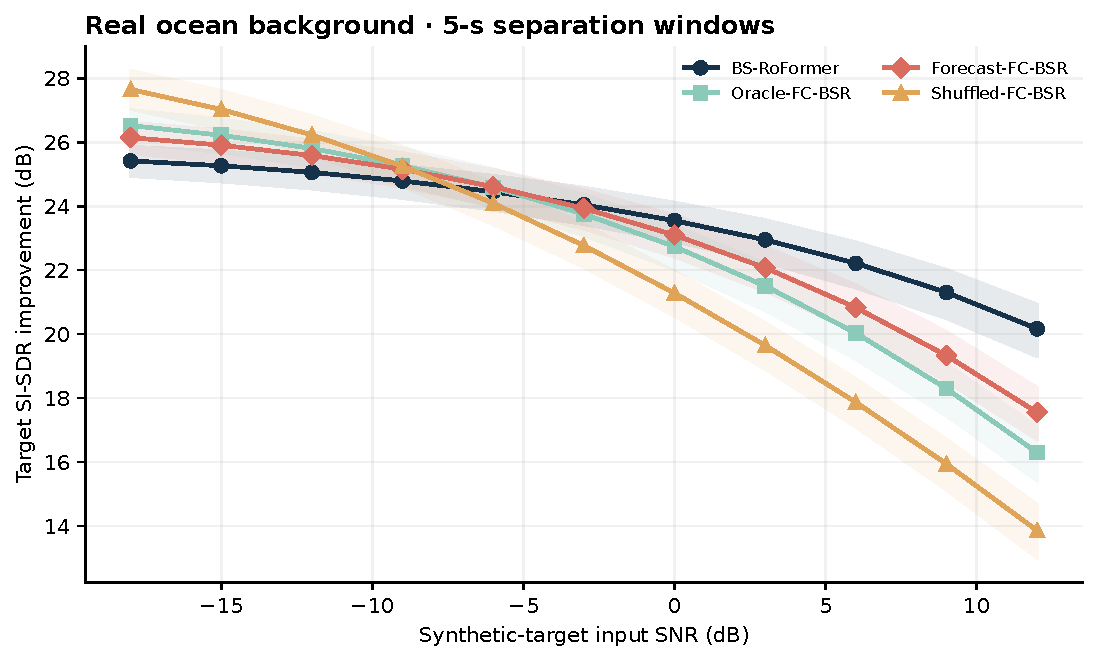
\includegraphics[width=\columnwidth]{figures/real_strength_sweep.pdf}
\caption{Ablation on 5-s unlabeled SanctSound background: target-strength
sweep.  Lines show the four conditions; shaded bands are paired 95\% intervals.}
\label{fig:strength}
\end{figure}

\begin{figure*}[t]
\centering
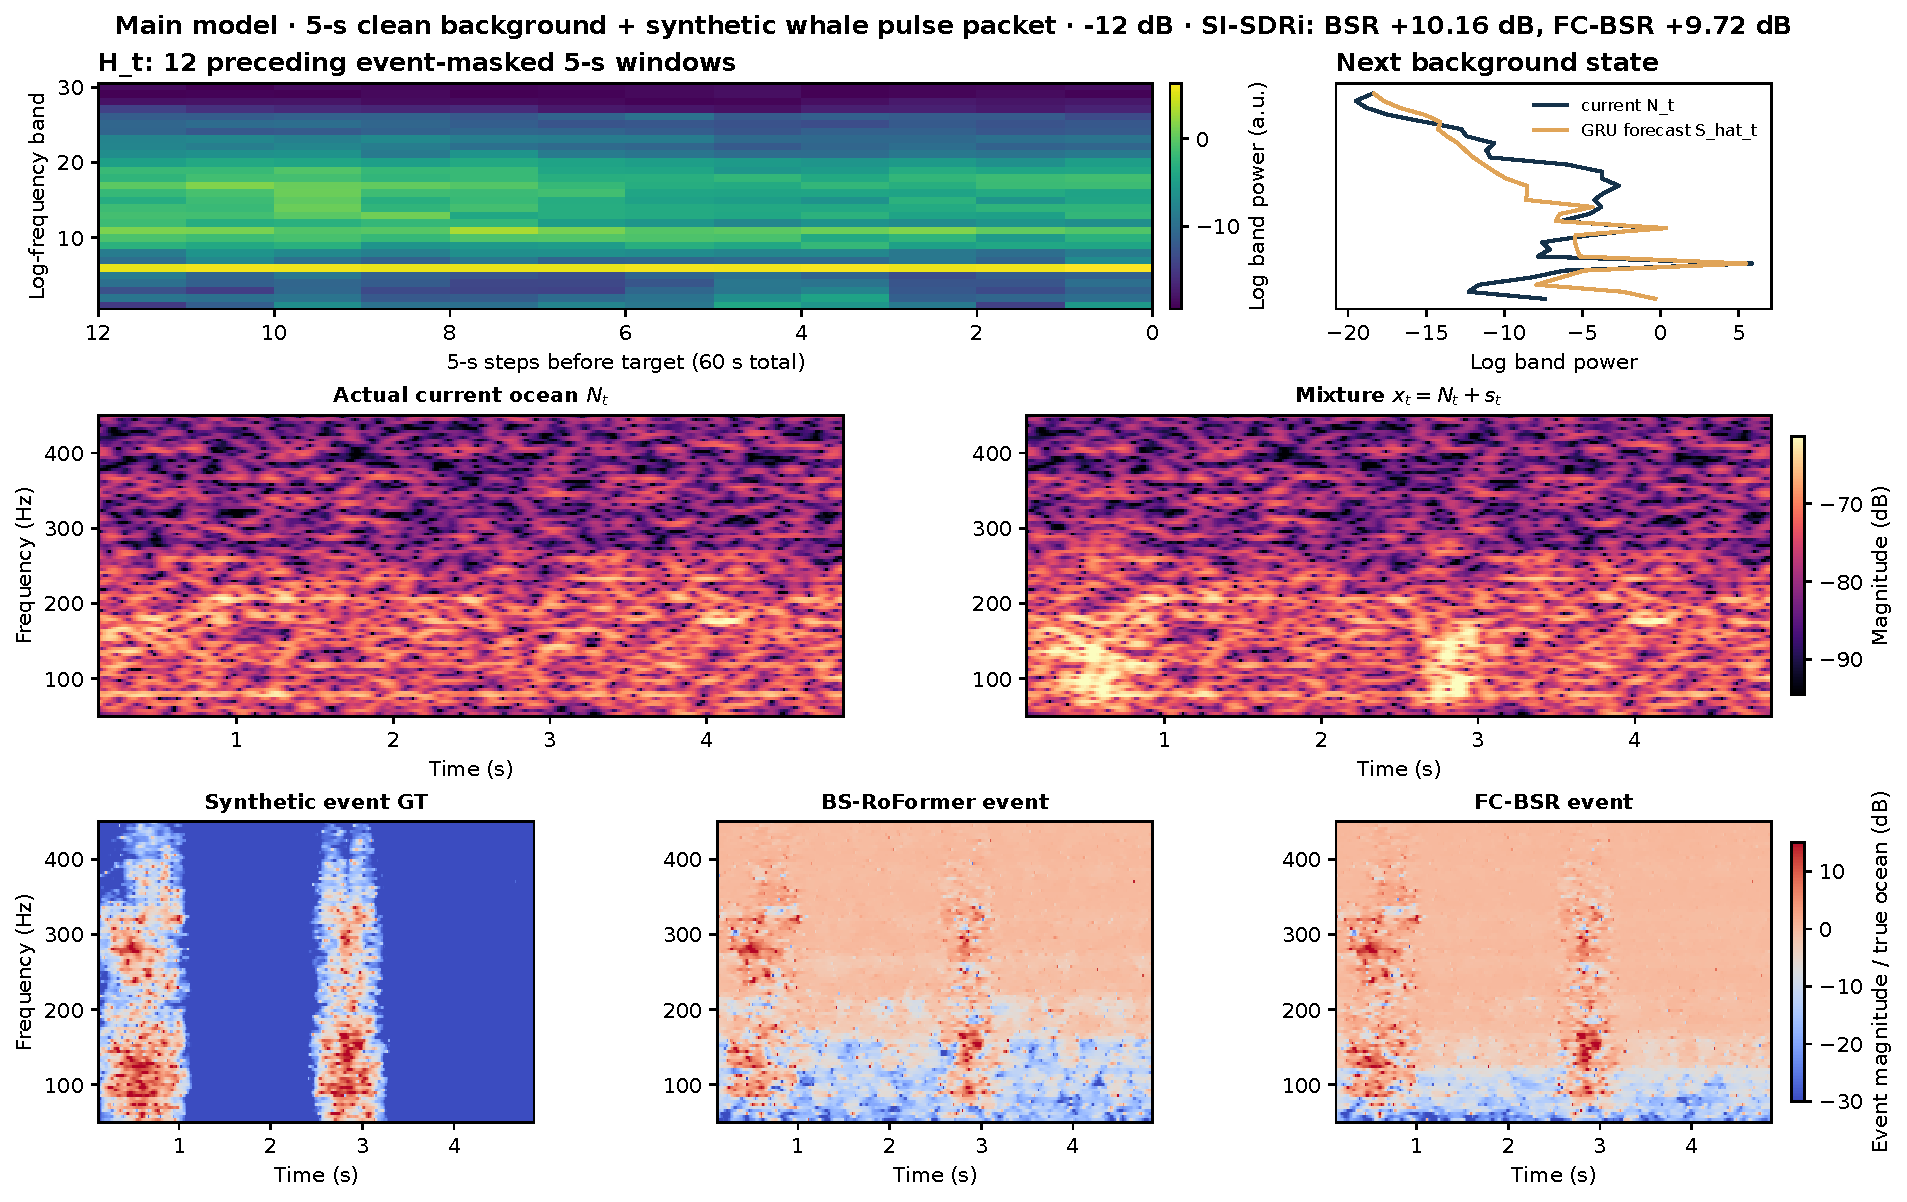
\includegraphics[width=.98\textwidth]{figures/real_audio_visualization.pdf}
\caption{Median-selected $-12$ dB synthetic whale pulse packet in a current
annotation-clean 5-s DCLDE recording.  All spectrograms share one magnitude
scale referenced to the mixture peak; the aggregate strength results are in
Fig.~\ref{fig:cleanstrength}.}
\label{fig:example}
\end{figure*}

\subsection{Real events without separated ground truth}
Following learned reference-free metrics \cite{kilgour2019fad,grais2019referenceless}
and semantic audio embeddings \cite{wu2023clap,xiao2024clapscore}, we train,
calibrate, and freeze a binary event classifier (test AUROC .9723, AP .9755,
F1 .9275).  Mixture consistency imposes $\hat N=x-\hat s$.  We restore
$\hat s$ at gains $\{-60,-30,-24,-18,-12,-6,0\}$ dB and test whether event
probability recovers monotonically.  Identity and all-to-event controls reject
trivial solutions; changes outside annotated intervals audit preservation.

The same frozen 12-step event-masked forecaster used by the main setting supplies
the causal history features.  Because recent call activity is masked, 103 real
test calls retain a full eligible 60-s history.  Table~\ref{tab:events} shows
the untouched-call results: FC-BSR trends toward lower residual event
probability and off-event change, while event-stem probability is nearly
unchanged.  The day-block intervals include zero for residual probability
$\Delta=-.0731$ ($[-.2090,.0294]$), event-stem probability $\Delta=+.0022$
($[-.0180,.0304]$), and monotonicity $\Delta=+.0178$ ($[-.0333,.0429]$).
Off-event relative error decreases by $.0248$ ($[-.0456,-.0018]$).  This small
semantic set is suggestive but not decisive; separated-stem ground truth is
still unavailable.

\begin{table*}[t]
\caption{Reference-free matched comparison on 103 real calls with eligible histories.}
\label{tab:events}\centering\footnotesize
\resizebox{\textwidth}{!}{%
\begin{tabular}{lrrrrr}
\toprule
Method &$p(x)$&$p(\hat N)\downarrow$&$p(\hat s)\uparrow$&Mono.$\uparrow$&Off-event$\downarrow$\\
\midrule
BS-RoFormer&.909&.786&.900&.937&.230\\
FC-BSR&.909&.713&.902&.955&.206\\
\bottomrule
\end{tabular}
}%
\end{table*}

\begin{figure}[t]
\centering
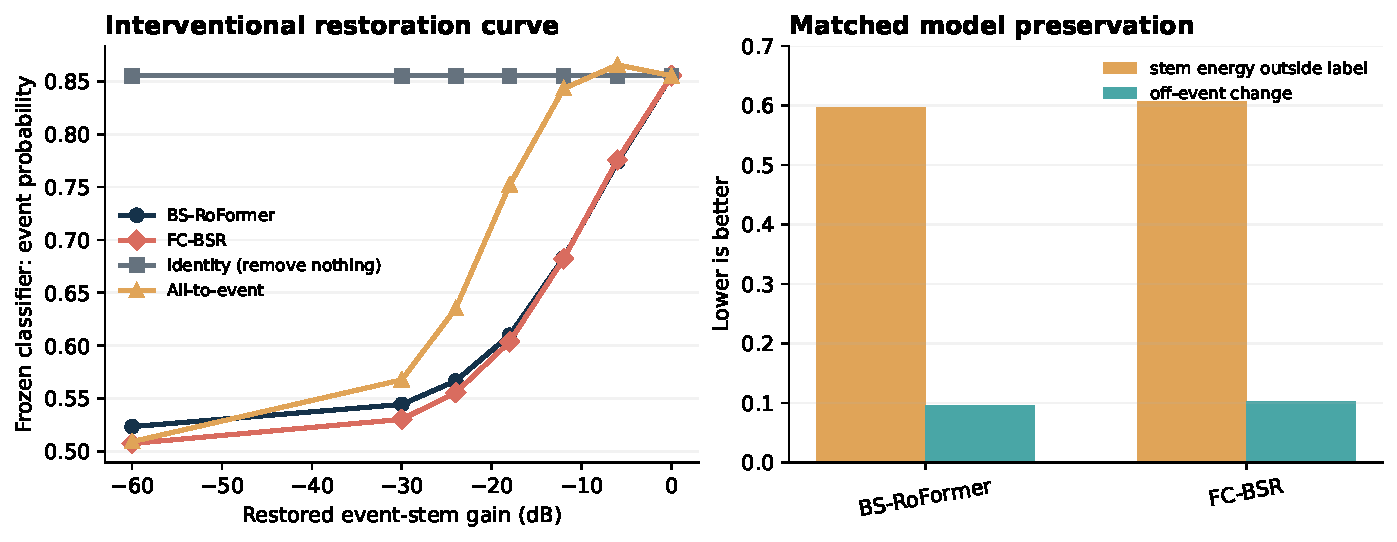
\includegraphics[width=\columnwidth]{figures/dclde_reference_free.pdf}
\caption{Reference-free restoration curves and preservation audit.  Both
models perform nontrivial semantic separation, but FC-BSR is not uniformly
better on real calls.}
\label{fig:real}
\end{figure}

\section{Discussion and Conclusion}
The evidence supports a narrower claim than the initial hypothesis.  On the
primary annotation-clean test, FC-BSR does not improve mean SI-SDRi over the
matched BS-RoFormer; the 95\% interval spans zero.  FiLM is
the best conditioning interface on controlled stems.  In the secondary
unannotated-WAV strength ablation, the prior helps weak targets, but that result
does not establish a gain on the annotation-clean main setting.  It is not universally beneficial: the gain
reverses for stronger targets, an oracle condition does not rescue the average,
and no decisive forecast advantage appears on untouched whale calls.  Persistence also
wins three of four predictor resolutions.  These negative controls are central:
they separate the existence of useful background information from a claim that
the present architecture always exploits it.

The local frontend is usable for inspection: on a CPU smoke test, one 5-s
chunk ran at RTF 0.014 after history features were prepared; the interface
displays forecasts and permits playback and download of both estimates.  This
does not establish field deployment.
Future work should condition only under calibrated uncertainty, test multiple
sites and seasons, and obtain isolated or stronger partial references for real
events.  Classifier-based restoration is evidence of semantic transfer, not a
replacement for waveform fidelity.

\clearpage
\balance
\bibliographystyle{IEEEtran}
\bibliography{reference}
\end{document}
